\section*{Materiale}

Il materiale utilizzato per questa esperienza di laboratorio è il sguente:

\begin{itemize} \itemsep2pt \parskip0pt \parsep0pt
    \item{Breadboard, cavetti e cavi a banana per le connessioni;}
    \item{Amplificatore operazionale UA741 a 8 pin;}
    \item{Resistenze da \SI{10}{\ohm} \SI{10}{\kilo\ohm} e \SI{100}{\kilo\ohm} ed una resistenza variabile tra $0$ e $10$ \SI{}{\kilo\ohm};}
    \item{Generatore di funzioni d'onda: Agilent 33120A;}
    \item{Multimetro: Agilent Technologies 34410A;}
    \item{Oscilloscopio: Agilent DSO-X 2002A;}
\end{itemize}

Facciamo presente che sui valori di resistenza riportati in tutto l'elaborato non abbiamo riportato la loro incertezza per motivi di chiarezza e leggibilità dello scritto. Tuttavia abbiamo assunto un errore del $5\%$ sul valore nominale delle resistenze.

\section*{Circuiti}

\begin{figure}[h]
        \centering
        \begin{subfigure}[b]{0.48\textwidth}
                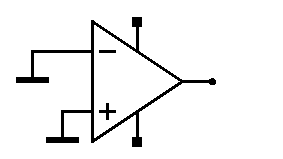
\includegraphics[width=\textwidth]{../figure/v_offset_exists.pdf}
                \caption{Amplificatore operazionale, configurazione open loop}
                \label{fig:open_loop}
        \end{subfigure}
        ~
        \begin{subfigure}[b]{0.48\textwidth}
                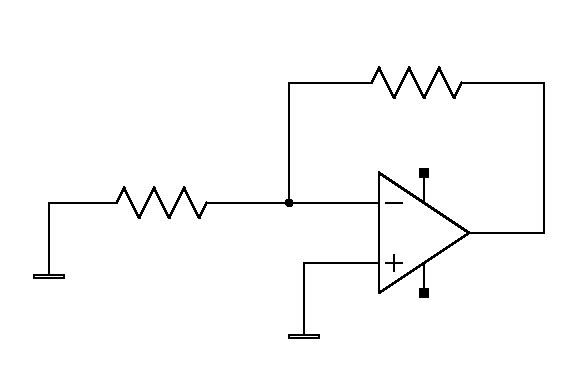
\includegraphics[width=\textwidth]{../figure/v_offset.pdf}
                \caption{Schema circuitale per la misura della tensione di offset}
                \label{fig:offset}
        \end{subfigure}
        \caption{Circuiti montati durante l'esperienza. Il primo ci permette di verificare il reale comportamento di un OPAMP, mentre il secondo ci permette di misurare/calcolare la tensione di offset.}
        \label{fig:circuits}
\end{figure}
